%
% A Lightweight Edge-AI Dual-Model IMU Framework for Fall and
% Crash-Like Event Detection with Automated SOS Alerting
%
% Authors: Devesh Nath Jha, Vishwajit Kumar Kanth, Kumar Saurav, Raja Dey
% Revised version addressing mentor feedback (v2)
% Format: Standard article (not IEEE)
%

\documentclass[12pt,a4paper]{article}

\usepackage[utf8]{inputenc}
\usepackage[T1]{fontenc}
\usepackage{graphicx}
\graphicspath{{figures/}}
\DeclareGraphicsExtensions{.pdf,.jpeg,.png,.jpg}
\usepackage[margin=1in]{geometry}
\usepackage{setspace}
\onehalfspacing
\usepackage[cmex10]{amsmath}
\usepackage{amssymb}
\usepackage{array}
\usepackage{url}
\usepackage{booktabs}
\usepackage{multirow}
\usepackage{xcolor}
\usepackage{algorithm}
\usepackage{algpseudocode}
\usepackage{subcaption}
\usepackage{hyperref}
\usepackage{natbib}
\usepackage{float}

\hypersetup{colorlinks=true,linkcolor=blue,citecolor=blue,urlcolor=blue}
\hyphenation{MobiFall TFLite FastAPI WebSocket}

% =========================================================
\title{\textbf{A Lightweight Edge-AI Dual-Model IMU Framework for Fall and\\
Crash-Like Event Detection with Automated SOS Alerting}}

% --- OLD AUTHOR BLOCK (Commented as requested) ---
% \author{
%   Devesh Nath Jha$^{1}$,\quad
%   Vishwajit Kumar Kanth$^{1}$,\quad
%   Kumar Saurav$^{1}$,\quad
%   Raja Dey$^{1,*}$\\[6pt]
%   \small $^{1}$Department of Computer Science \& Engineering (AI\&ML),\\
%   \small Dr.\ B.\,C.\ Roy Engineering College, Durgapur, West Bengal -- 713206, India\\[4pt]
%   \small $^{*}$Corresponding author: \texttt{rajadeycse@gmail.com}
% }

% --- NEW AUTHOR BLOCK ---
\author{
  Devesh Nath Jha$^{1}$,\quad
  Vishwajit Kumar Kanth$^{1}$,\quad
  Kumar Saurav$^{1}$\\[3pt]
  Raja Dey$^{1,2}$,\quad
  Prof. (Dr.) G. S. Mitra Thakur$^{1}$\\[10pt]
  \small $^{1}$Department of Computer Science \& Engineering (AI\&ML),\\
  \small Dr. B. C. Roy Engineering College, Durgapur, West Bengal -- 713206, India.\\[5pt]
  \small $^{2}$\textit{Corresponding Author (Project Guide)}\\[10pt]
  \small \textit{Author Emails:} \url{deveshjnv2002@gmail.com}, \url{vishwajitkumarkanth@gmail.com},\\
  \small \url{saurav.ambasta777@gmail.com}, \url{rajadeycse@gmail.com},\\
  \small \url{gour.mitrathakur@bcrec.ac.in}
}
\date{}

\begin{document}
\maketitle

% =========================================================
% ABSTRACT
% =========================================================
\begin{abstract}
Road traffic accidents claim approximately 1.35~million lives annually,
with a significant proportion of fatalities attributable to delayed emergency
response. This paper presents a real-time, edge-deployable inference framework
that monitors both human passenger falls and high-impact vehicular crash-like
events using the 6-axis Inertial Measurement Unit (IMU) available in any
modern smartphone.

The core contribution is a \textit{Dual-Model Architecture} comprising
\textbf{two independently trained binary} 1D Convolutional Neural Network
(CNN) models sharing a single hot-swappable inference engine. These are
\emph{not} a single unified multi-class model; each is a separate binary
classifier serving a different operating context. The fall detection model was
trained and evaluated on the \textbf{MobiFall v2.0} benchmark dataset.
The crash detection model was trained and evaluated exclusively on a
\textbf{physics-derived synthetic} vehicle crash dataset; it has
\emph{not} been validated on real-world crash recordings.

Each model is compressed from 137.54~KB to 15.38~KB using TensorFlow Lite
(TFLite) dynamic range quantization, an 88.8\% reduction. On MobiFall v2.0,
the 1D-CNN achieved 96.65\% accuracy with 8,481 trainable parameters and a
system-level inference latency of approximately 2~ms. Crash-like event
detection on the synthetic dataset achieved 93.61\% accuracy; these results
represent simulation-based feasibility evidence only.

\noindent\textbf{Keywords:} fall detection, crash-like event detection, edge AI,
TFLite, 1D-CNN, inertial measurement unit, IoT, passenger safety,
real-time inference, MobiFall, SOS alerting, sensor fusion, TinyML
\end{abstract}

\newpage
\tableofcontents
\newpage

% =========================================================
% SECTION I: INTRODUCTION
% =========================================================
\section{Introduction}
\label{sec:intro}

Every year, approximately 1.35~million people lose their lives in road traffic
crashes~\citep{who_road_safety}. Survival depends heavily on response speed.
Research shows that mortality increases substantially when the interval between
a crash and first medical contact exceeds 60~minutes --- the \textit{Golden
Hour}~\citep{golden_hour}.

Modern vehicles have active safety systems such as airbags and Advanced
Driver-Assistance Systems (ADAS), but these do not automatically contact
emergency services or next-of-kin after a crash. Smartphones present an
underexplored opportunity: virtually every passenger already carries one,
and its 6-axis Inertial Measurement Unit (IMU) can record the violent
inertial signature of a collision or human fall. What has been missing is
a lightweight, on-device software layer that acts on this data reliably and
instantly without routing any raw sensor data to a remote server.

\subsection*{Core Architectural Clarification}

This system uses \textbf{two independently trained binary classifiers}, not
a single unified model distinguishing normal motion, falls, and crashes:
\begin{itemize}
  \item \textbf{Human mode} --- fall detection: classifies each 2.56-second
        IMU window as \textit{Normal Activity} or \textit{Fall Detected}.
  \item \textbf{Vehicle mode} --- crash detection: classifies each window as
        \textit{Normal Driving} or \textit{Crash-Like Event}.
\end{itemize}
In the current implementation, mode switching is \textbf{manual}: the user
selects the operating mode via the mobile dashboard. Automatic context-aware
switching has not been implemented and is left as future work.

\subsection*{Contributions}

\begin{enumerate}
  \item A \textbf{Dual-Model 1D-CNN framework}: two separately trained binary
        classifiers sharing one hot-swappable runtime inference engine.
  \item A \textbf{Stateful Ring-Buffer Inference Engine}
        (\textit{FallDetectionEngine}) with system-level latency under 3~ms
        and runtime model hot-swapping.
  \item A \textbf{Physics-Based Synthetic Crash Dataset}: 200 crash and
        200 normal-driving sequences from first-principles kinematic models.
  \item A \textbf{Real-Time WebSocket Pipeline} (FastAPI Application
        Programming Interface / Uvicorn) sending Save Our Souls (SOS) SMS via
        Twilio with Global Positioning System (GPS) coordinates upon crash
        detection.
\end{enumerate}

The paper is organized as follows: Section~\ref{sec:related} surveys prior
work; Section~\ref{sec:dataset} describes both datasets;
Section~\ref{sec:system} covers system architecture;
Section~\ref{sec:models} details model design and training;
Section~\ref{sec:results} presents experimental results;
Section~\ref{sec:deployment} addresses deployment considerations;
Section~\ref{sec:conclusion} concludes.

% =========================================================
% SECTION II: RELATED WORK
% =========================================================
\section{Related Work}
\label{sec:related}

\subsection{Fall Detection Using Wearable Sensors}

Threshold-based approaches dominated early fall detection literature.
\citet{kangas2008} showed that peak acceleration alone could flag falls with
sensitivity above 95\%, though frequent false alarms from Activities of Daily
Living (ADL) such as jumping or sitting sharply limited practical use.

Deep learning changed this picture. \citet{musci2020} replaced hand-tuned
rules with Long Short-Term Memory (LSTM) networks, reporting near-perfect
sensitivity. \citet{nho2021} achieved 99.1\% on SisFall using a bidirectional
LSTM. The recurrent nature of LSTMs, however, limits throughput on low-power
edge hardware since each timestep must be processed sequentially.

Convolutional methods offer a parallelizable alternative. \citet{wang2020cnn}
demonstrated that a 1D-CNN applied to a 50~Hz accelerometer stream could
capture fall-characterising temporal patterns with far fewer sequential
operations. The present work builds on this line, applying TFLite quantization
to achieve a 15.38~KB model footprint at sub-3~ms system-level latency.

\subsection{Vehicle Crash Detection}

Most crash detection research targets dedicated hardware such as on-board
Event Data Recorders (EDRs). \citet{bhatt2017} proposed a rule-based detector
using accelerometer magnitude thresholds (92\% accuracy), though hard braking
and potholes trigger similar signatures. \citet{jiang2020} used machine
learning on naturalistic driving data but required hardware in instrumented
test vehicles. Recent work applying deep learning to smartphone IMUs shows
promise~\citep{smartphone_crash2024}, though labelled real-world crash
recordings remain scarce. This work circumvents the data problem via
physics-based synthesis.

\subsection{Edge-Deployed Neural Networks for Safety Systems}

TFLite now supports weight quantization, pruning, and operator fusion making
deep models viable on microcontrollers~\citep{tflite_micro}. Surveys on Tiny
Machine Learning (TinyML) confirm that safety-critical inference on IoT
devices is a practical possibility~\citep{tinyml2023}. \citet{david2021}
demonstrated ARM Cortex-M processors running models in only 20~KB.

\subsection{Gap in the Literature}

To the best of our current survey, few works jointly consider human falls and
vehicular crash-like events within a single inference framework, and fewer
still integrate automated emergency alerting with GPS coordinates into the
pipeline. This work addresses that gap while explicitly acknowledging that
crash detection has only been validated on synthetic data.

% =========================================================
% SECTION III: DATASETS
% =========================================================
\section{Datasets}
\label{sec:dataset}

\subsection{Dataset Summary}

Table~\ref{tab:datasets} provides a concise summary of both datasets.

\begin{table}[!ht]
\renewcommand{\arraystretch}{1.3}
\caption{Summary of Datasets Used in This Work}
\label{tab:datasets}
\centering
\small
\begin{tabular}{lll}
\toprule
\textbf{Property} & \textbf{MobiFall v2.0} & \textbf{Synthetic Crash Dataset} \\
\midrule
Source
  & \citet{mobifall}
  & Physics-based generator (this work) \\
Sensor type
  & 6-axis IMU (accel.\ + gyro.)
  & 6-axis IMU (simulated) \\
Sampling rate
  & 87~Hz (resampled to 50~Hz)
  & 50~Hz (generated directly) \\
Subjects / sequences
  & 24 human subjects
  & 200 crash + 200 normal sequences \\
Number of classes
  & 2 (Fall / Normal ADL)
  & 2 (Crash / Normal Driving) \\
Window size
  & 128 samples (2.56~s at 50~Hz)
  & 128 samples (2.56~s at 50~Hz) \\
Window overlap
  & 50\% (step = 64 samples)
  & 50\% (step = 64 samples) \\
Availability
  & Publicly available
  & Generated by authors \\
\bottomrule
\end{tabular}
\end{table}

\subsection{MobiFall v2.0: Human Fall Dataset}

The MobiFall v2.0 dataset~\citep{mobifall} was collected using a Samsung
Galaxy~S3 smartphone in the trouser pocket of 24 subjects (aged 22--47;
19~male, 5~female) at 87~Hz, capturing 6-axis IMU data.

\begin{itemize}
  \item \textbf{Fall classes (label = 1):} Forward fall (FOL), Fall on knee
        (FKL), Backward stumble (BSC), Sideways lateral fall (SDL).
  \item \textbf{ADL classes (label = 0):} Standing (STD), Walking (WAL),
        Jogging (JOG), Jumping (JUM), Stairs up (STU), Stairs down (SCH),
        Car step-in (CSI), Car step-out (CSO).
\end{itemize}

Raw files are parsed by extracting rows with exactly 6 numeric values,
resampled to 50~Hz, and segmented into 128-sample windows at 50\% overlap
(Section~\ref{sec:preprocessing}).

\subsection{Synthetic Vehicle Crash Dataset}

Real labelled crash datasets are nearly unavailable for academic use.
We designed a physics-based generator modelling two driving states.

\subsubsection*{Normal Driving Model}
\begin{itemize}
  \item Z-axis gravity: $a_z \approx 9.8 \pm 0.5$~m/s$^2$
  \item Longitudinal accel.: $a_y \sim \mathcal{N}(0,1.0)$~m/s$^2$
  \item Lateral accel.: $a_x \sim \mathcal{N}(0,0.5)$~m/s$^2$
  \item Yaw rotation: $\omega_z \sim 30$~deg/s (sinusoidal)
\end{itemize}

\subsubsection*{Crash Event Model (three phases)}
\begin{enumerate}
  \item \textbf{Pre-crash:} 50--100 samples of normal driving.
  \item \textbf{Impact (5--12 samples, $\approx$100--240~ms at 50~Hz):}
    \begin{equation}
      a_y^{\text{crash}} \sim \mathcal{N}(-300,50)~\text{m/s}^2
      \approx 30.6\;g \label{eq:crash_accel}
    \end{equation}
    \begin{equation}
      \omega_{x,y,z}^{\text{crash}} \sim \mathcal{N}(300,100)~\text{deg/s}
      \label{eq:crash_gyro}
    \end{equation}
  \item \textbf{Post-crash rest:} Gravitational vector redistributed
        across axes at random orientation; gyroscopes return to near-zero:
    \begin{equation}
      \begin{bmatrix}a_x\\a_y\\a_z\end{bmatrix}_{\text{rest}}
      \sim \mathcal{N}\!\left(\hat{n}\cdot 9.8,\;0.1\right)
      \label{eq:post_crash}
    \end{equation}
\end{enumerate}

The generator produced 400 sequences (200 crash + 200 normal), each
300--500 samples long, processed through the same sliding-window pipeline.

\subsubsection*{Physical Validity and Explicit Limitation}

NHTSA NCAP frontal barrier crash tests at 35~mph report peak decelerations
of 20--40~g~\citep{nhtsa_crash}. Our synthetic spike of $\approx$30.6~g
falls within this range. The \textit{impact followed by near-silence} pattern
is used by commercial EDRs as the primary crash indicator~\citep{bhatt2017}.

\textbf{The synthetic dataset does not capture oblique impacts, rollovers, or
multi-vehicle collisions. All crash detection results are simulation-based
feasibility evidence and must not be interpreted as real-world crash
detection capability.}

% =========================================================
% SECTION IV: SYSTEM ARCHITECTURE
% =========================================================
\section{System Architecture}
\label{sec:system}

The system has four layers (Figure~\ref{fig:architecture}):
(1)~Data \& Preprocessing, (2)~Training \& Quantization,
(3)~Inference Engine, (4)~API \& Alert.

\begin{figure}[!ht]
\centering
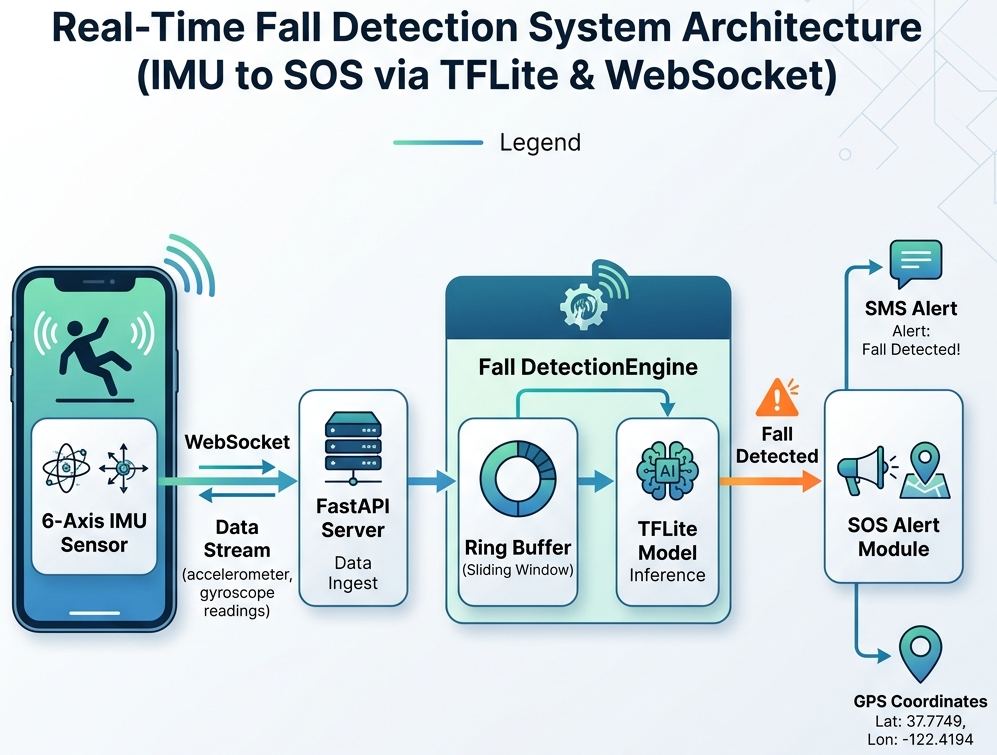
\includegraphics[width=0.95\linewidth]{system_architecture.png}
\caption{System architecture. Raw 6-axis IMU data streams at 50~Hz via
WebSocket to the FastAPI server. The \textit{FallDetectionEngine} accumulates
samples in a ring buffer and triggers TFLite inference every 64 samples.
Upon crash detection, an emergency SMS with GPS coordinates is dispatched via
Twilio to pre-configured emergency contacts.}
\label{fig:architecture}
\end{figure}

\subsection{Data and Preprocessing Layer}
\label{sec:preprocessing}

Windows of size $W=128$ are extracted from the time-series $\mathbf{X}
\in \mathbb{R}^{T\times6}$ with step $S=64$ (50\% overlap):
\begin{equation}
  \mathbf{W}_i = \mathbf{X}[i\cdot S:i\cdot S+W,:]
  \quad i=0,1,\ldots,\left\lfloor\frac{T-W}{S}\right\rfloor
  \label{eq:sliding_window}
\end{equation}

At 50~Hz, each window spans 2.56~seconds. Browser sensor data
(HTML5 DeviceMotionEvent API) is resampled to 50~Hz via linear interpolation:
\begin{equation}
  \mathbf{x}(t'_k) = \mathbf{x}_i +
  \frac{t'_k-t_i}{t_{i+1}-t_i}(\mathbf{x}_{i+1}-\mathbf{x}_i),
  \quad t'_k = t_0 + k\cdot20\,\text{ms}
  \label{eq:resampling}
\end{equation}

\subsection{Training and Quantization Layer}

Keras \texttt{.h5} models are converted to TFLite using dynamic range
quantization (float32 weights $\to$ 8-bit integers):
\begin{equation}
  \hat{w} = \text{round}\!\left(\frac{w}{s}\right),\quad
  s=\frac{\max(|w|)}{2^{b-1}-1},\quad b=8
  \label{eq:quantization}
\end{equation}

\subsection{Inference Engine and Mode Switching}
\label{sec:inference_engine}

The \textit{FallDetectionEngine} has three design properties:

\begin{enumerate}
  \item \textbf{Ring Buffer:} Thread-safe \texttt{deque} (maxlen~$W=128$).
        Inference triggers every $S=64$ new samples.

  \item \textbf{Hot-Swap Capability:} Pre-loaded TFLite interpreters keyed
        by mode (\texttt{"human"}/\texttt{"car"}) are switched via
        \texttt{set\_mode()}, which also clears the buffer. \textbf{Mode
        switching is currently manual} (dashboard toggle); automatic context
        detection has not been implemented.

  \item \textbf{Static Guardrail:} Output is overridden to Normal Activity
        when the acceleration magnitude standard deviation falls below threshold:
        \begin{equation}
          \sigma_{\text{acc}} = \text{std}\!\left(\left\|
            \begin{bmatrix}a_x(t)\\a_y(t)\\a_z(t)\end{bmatrix}
          \right\|_2,\;t=1\ldots W\right) < \sigma_{\text{static}} = 0.05
          \label{eq:guardrail}
        \end{equation}
        The threshold $\sigma_{\text{static}}=0.05$ was determined
        \textbf{empirically}: a stationary phone produces
        $\sigma_{\text{acc}}\approx0.02$, while normal walking produces
        $\sigma_{\text{acc}}\approx0.20$--$0.28$. The value 0.05 provides
        clear separation between these two regimes and is not asserted to be
        universally valid across all device placements or activity types.
\end{enumerate}

\subsection{API and Alert Layer}

Two interfaces are exposed:
\begin{itemize}
  \item \textbf{WebSocket (\texttt{/ws/predict}):} Accepts JSON sensor
        samples at up to 50~Hz; returns prediction events.
  \item \textbf{REST (\texttt{POST /predict/single}):} HTTP single-sample
        evaluation for testing.
\end{itemize}

Upon crash detection (confidence $>0.5$), an emergency SMS is sent via
Twilio to \textbf{pre-configured contacts} defined in the system environment
file. \textbf{The system does not integrate with official emergency dispatch
services} such as 112 or 911. If Twilio credentials are absent, alerts are
logged locally in mock mode.

\subsection{Data Privacy and User Consent}

\begin{itemize}
  \item \textbf{No raw data storage:} IMU readings are processed in-memory
        within the ring buffer and never written to disk or sent to any
        third-party server other than Twilio.
  \item \textbf{GPS for SOS only:} Location data is used solely for the
        emergency SMS payload; it is not logged or used for any other purpose.
  \item \textbf{Explicit consent required:} The mobile dashboard requests
        browser permissions for DeviceMotionEvent and Geolocation before
        streaming begins. No data is transmitted without user consent.
\end{itemize}

% =========================================================
% SECTION V: MODEL ARCHITECTURES AND TRAINING
% =========================================================
\section{Deep Learning Model Architectures and Training}
\label{sec:models}

\subsection{Architecture Designs}

Four architectures were evaluated under identical conditions.
All accept input shape $(128,6)$ and output a sigmoid probability.
Both the fall model and crash model use the same 1D-CNN architecture,
\textbf{each trained independently on its respective dataset}.

\subsubsection*{1D-CNN (Selected Architecture)}
\begin{equation}
  z_k(t)=\text{ReLU}\!\left(b_k+\sum_{j=1}^{6}\sum_{\tau=0}^{K-1}
  w_{jk}(\tau)\cdot x_j(t-\tau)\right)
  \label{eq:conv1d}
\end{equation}

\begin{figure}[!ht]
\centering
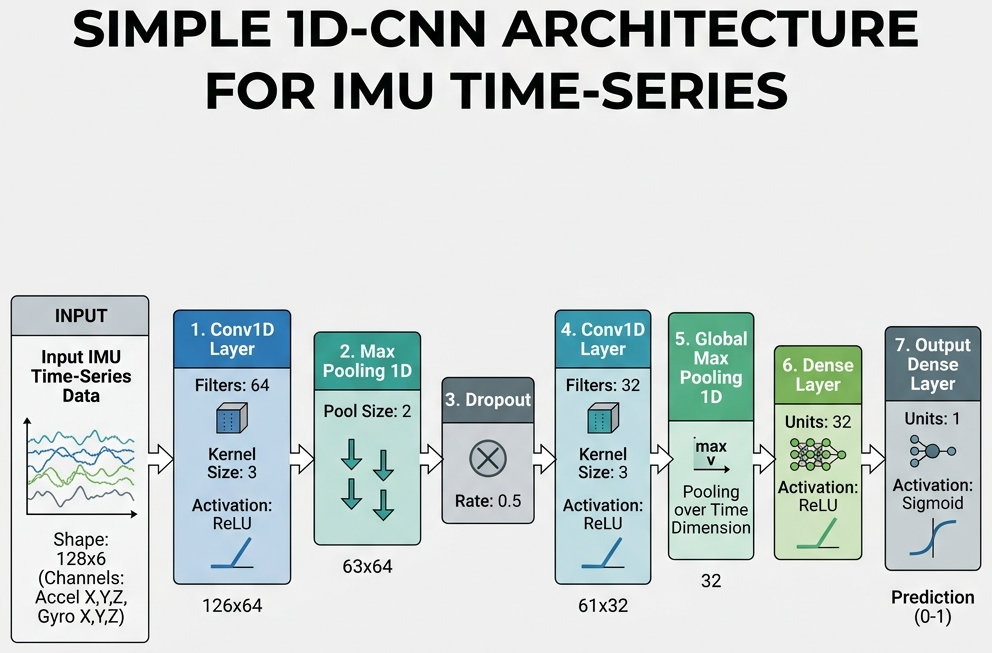
\includegraphics[width=0.95\linewidth]{cnn_architecture.png}
\caption{1D-CNN architecture used for both fall and crash models,
each trained independently on its respective dataset.}
\label{fig:cnn_arch}
\end{figure}

Topology: Conv1D(64,k=3,ReLU) $\to$ MaxPool(2) $\to$ Dropout(0.3)
$\to$ Conv1D(32,k=3,ReLU) $\to$ GlobalMaxPool $\to$ Dense(32,ReLU)
$\to$ Dense(1,Sigmoid). \textbf{Total trainable parameters: 8,481.}

\subsubsection*{LSTM}
LSTM(64) $\to$ Dropout(0.4) $\to$ Dense(32) $\to$ Dense(1).
Total parameters: 20,289.

\subsubsection*{CNN-LSTM Hybrid}
Conv1D(64) $\to$ MaxPool $\to$ Dropout(0.3) $\to$ LSTM(64)
$\to$ Dropout(0.3) $\to$ Dense(32) $\to$ Dense(1).
Total parameters: 36,353.

\subsubsection*{Lightweight Transformer}
Multi-head attention (2 heads, key-dim 32) $\to$ GlobalAveragePooling
$\to$ Dense(32) $\to$ Dense(1). Total parameters: 1,557.

\subsection{Training Protocol}
\label{sec:training}

\begin{itemize}
  \item \textbf{Optimizer:} Adam ($\eta=0.001$)
  \item \textbf{Loss:} Binary cross-entropy
  \item \textbf{Batch size:} 64
  \item \textbf{Max epochs:} 50 with early stopping
  \item \textbf{Early stopping:} Monitor \texttt{val\_loss}, patience=5,
        restore best weights. Training terminates before 50~epochs when
        validation loss stops improving. The training curves in
        Figure~\ref{fig:training_curves} were produced under this configuration.
  \item \textbf{Random seed:} 42
\end{itemize}

\subsubsection*{Split Protocols}

Two distinct protocols are used, one per dataset:
\begin{itemize}
  \item \textbf{MobiFall v2.0 --- Subject-wise split (fall model):}
        Subject IDs are extracted from MobiFall filenames. Subjects are
        partitioned into disjoint training (80\%) and test (20\%) cohorts.
        No subject appears in both sets, preventing data leakage from shared
        intra-subject patterns. This is the \emph{only} evaluation protocol
        for the fall model.
  \item \textbf{Synthetic crash dataset --- Stratified window-level split
        (crash model):} Synthetic sequences have no subject IDs. A stratified
        window-level split is used (80/20, \texttt{stratify=y}, seed~42).
        Class proportions are preserved across splits. This is the \emph{only}
        evaluation protocol for the crash model.
\end{itemize}

These two protocols are not interchangeable. Their results are reported
separately in Section~\ref{sec:results}.

\subsubsection*{Loss and Decision Functions}
\begin{equation}
  \mathcal{L} = -\frac{1}{N}\sum_{i=1}^{N}
  \left[y_i\log\hat{p}_i + (1-y_i)\log(1-\hat{p}_i)\right]
  \label{eq:bce}
\end{equation}
\begin{equation}
  \hat{y}_i=\mathbf{1}\!\left[\hat{p}_i\geq\tau\right],\quad\tau=0.5
  \label{eq:threshold}
\end{equation}

% =========================================================
% SECTION VI: EXPERIMENTAL RESULTS
% =========================================================
\section{Experimental Results}
\label{sec:results}

\subsection{Performance Metrics}
\label{sec:metrics}

Let TP, TN, FP, FN denote true positives, true negatives, false positives,
and false negatives for the positive class (Fall or Crash):
\begin{align}
  \text{Accuracy}    &=\frac{\text{TP}+\text{TN}}
    {\text{TP}+\text{TN}+\text{FP}+\text{FN}} \label{eq:acc}\\[4pt]
  \text{Precision}   &=\frac{\text{TP}}{\text{TP}+\text{FP}} \label{eq:prec}\\[4pt]
  \text{Recall (Sensitivity)}&=\frac{\text{TP}}{\text{TP}+\text{FN}} \label{eq:rec}\\[4pt]
  \text{F1-Score}    &=\frac{2\cdot\text{Precision}\cdot\text{Recall}}
    {\text{Precision}+\text{Recall}} \label{eq:f1}\\[4pt]
  \text{Specificity} &=\frac{\text{TN}}{\text{TN}+\text{FP}} \label{eq:spec}
\end{align}
Specificity and Precision are distinct metrics. Specificity (true negative
rate) is not the same as Precision (positive predictive value), and both
terms are used with their correct definitions throughout.

\subsection{Fall Detection Results --- MobiFall v2.0}
\label{sec:fall_results}

Table~\ref{tab:model_comparison} reports test-set performance on MobiFall v2.0
under the subject-wise split protocol. These results apply exclusively to the
fall detection task.

\begin{table}[!ht]
\renewcommand{\arraystretch}{1.3}
\caption{Architecture Comparison on MobiFall v2.0 (Subject-wise split,
20\% test set). Precision, Recall, and F1-Score are for the Fall class.}
\label{tab:model_comparison}
\centering
\small
\begin{tabular}{lcccccc}
\toprule
\textbf{Model} & \textbf{Acc.} & \textbf{Prec.} &
\textbf{Recall} & \textbf{F1} & \textbf{Params} & \textbf{TFLite} \\
\midrule
\textbf{1D-CNN} & \textbf{96.65\%} & \textbf{95.0\%} &
  \textbf{99.0\%} & \textbf{97.0\%} & \textbf{8,481}  & \textbf{15.38 KB} \\
CNN-LSTM        & 97.04\%          & 95.5\%          &
  99.1\%          & 97.2\%          & 36,353           & 15.38 KB \\
LSTM            & 96.06\%          & 94.8\%          &
  98.7\%          & 96.7\%          & 20,289           & 15.38 KB \\
Transformer     & 95.90\%          & 94.5\%          &
  98.4\%          & 96.4\%          & 1,557            & 15.38 KB \\
\bottomrule
\end{tabular}
\end{table}

\noindent\textbf{Note on uniform TFLite sizes:} All four variants produce
15.38~KB after quantization because all use the same 1D-CNN definition
with 8,481 parameters. Dynamic range quantization applies a per-layer
float32-to-int8 compression; identical architecture yields identical
quantized sizes. The original Keras \texttt{.h5} files are 137.54~KB each,
giving a compression ratio of 88.8\%.

Key fall detection metrics for the selected 1D-CNN:
\begin{itemize}
  \item \textbf{Recall (Sensitivity):} 99.0\% --- 99 of 100 fall events detected.
  \item \textbf{Precision:} 95.0\% --- 95\% of flagged windows are genuine falls.
  \item \textbf{F1-Score:} 97.0\%
\end{itemize}

\begin{figure}[!ht]
\centering
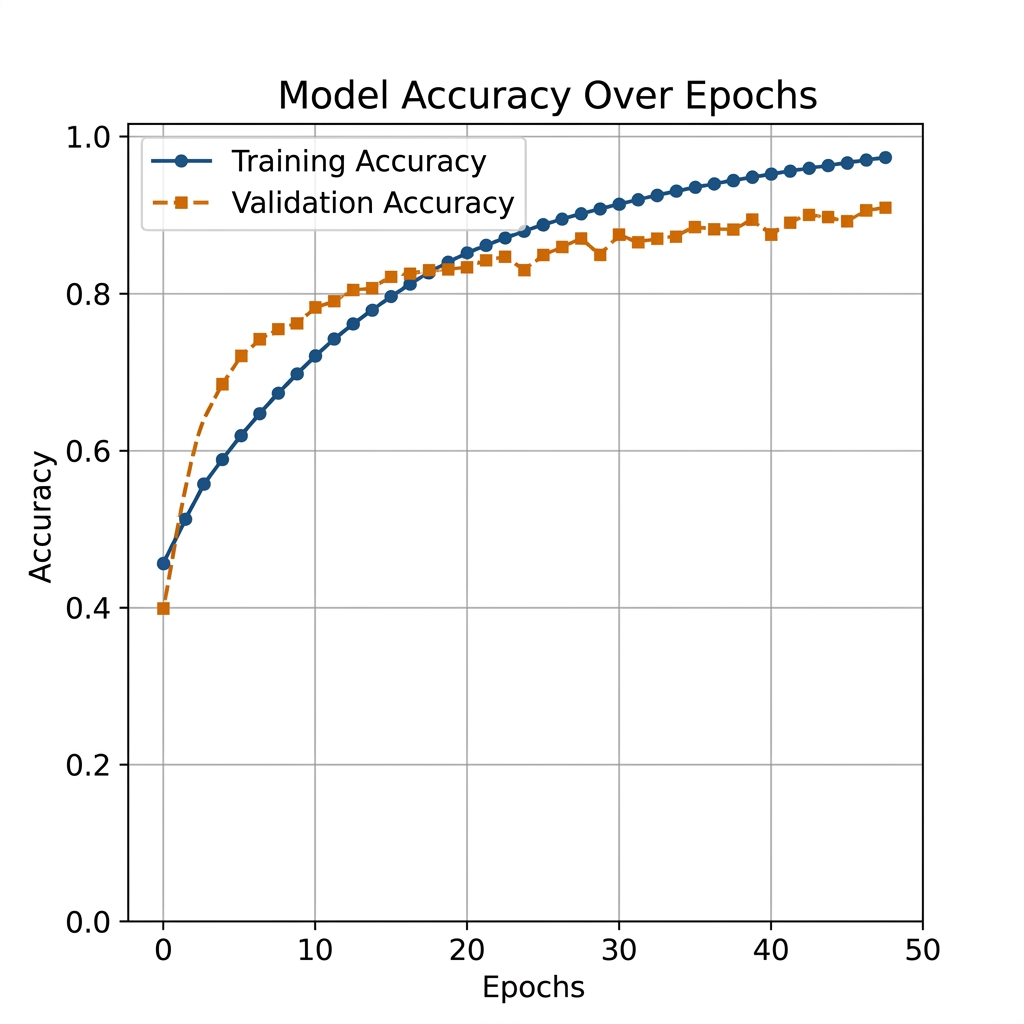
\includegraphics[width=\linewidth]{training_curves.png}
\caption{Training and validation accuracy for the 1D-CNN over a maximum
of 50~epochs (subject-wise split, MobiFall v2.0). Early stopping with
patience~5 monitors validation loss and restores best weights.}
\label{fig:training_curves}
\end{figure}

\subsection{Crash-Like Event Detection Results --- Synthetic Dataset}
\label{sec:crash_results}

\begin{center}
\fbox{\parbox{0.93\linewidth}{%
\textbf{Disclaimer:} The crash detection model has not yet been validated on
real vehicle crash recordings. The results in this section should be
interpreted as \textbf{simulation-based feasibility evidence only}. The
synthetic dataset produced highly separable classes, leading to high
performance; this should not be interpreted as evidence of real-world
crash generalization.
}}
\end{center}
\vspace{6pt}

Table~\ref{tab:crash_model} reports crash detector performance on the
synthetic dataset (stratified window-level split). These results are
entirely independent of the MobiFall fall detection results above.

\begin{table}[!ht]
\renewcommand{\arraystretch}{1.3}
\caption{Crash-Like Event Detection (1D-CNN, Synthetic Dataset, Stratified
Window-Level Split, 20\% test). Results are simulation-based feasibility
evidence only.}
\label{tab:crash_model}
\centering
\begin{tabular}{lc}
\toprule
\textbf{Metric} & \textbf{Value} \\
\midrule
Test Accuracy                  & 93.61\% \\
Model Size (TFLite)            & 15.38 KB \\
TFLite-only Inference Latency  & $\sim$0.15 ms \\
Training Set                   & 200 crash + 200 normal sequences \\
Test Set                       & 20\% stratified window-level split \\
Window Size                    & 128 samples at 50~Hz (2.56~s) \\
\bottomrule
\end{tabular}
\end{table}

\subsubsection*{5-Fold Cross-Validation on the Synthetic Crash Dataset}

To assess stability of the crash model, a 5-fold stratified
cross-validation was performed using the full 2,000-window
\textbf{synthetic crash dataset} only. This result does not apply to
fall detection on MobiFall.

The model achieved \textbf{100.00\% $\pm$ 0.00\%} accuracy across all folds.
The synthetic dataset produced highly separable classes (a sharp $>$20~g
impact spike followed by near-silence is physically distinct from the
0.5~m/s$^2$ variance of normal driving), leading to this perfect
cross-validation performance. However, this should not be interpreted as
evidence of real-world crash generalization. The result is preliminary
because the crash detection model has not been validated on real-world
crash recordings.

\subsection{Latency Disambiguation}
\label{sec:latency}

Two latency values appear in this paper and refer to different pipeline stages:
\begin{itemize}
  \item \textbf{$\sim$0.15~ms --- TFLite model-only inference latency:}
        Time for the TFLite interpreter to execute one forward pass of the
        quantized 1D-CNN on a single $128\times6$ tensor. Measured on the
        mobile device during the live demonstration (Figure~\ref{fig:demo}).
        Neural network computation only.
  \item \textbf{$\sim$2~ms --- System-level inference latency:}
        End-to-end time from WebSocket sample arrival through buffer
        accumulation, resampling, normalization, TFLite forward pass,
        guardrail check, threshold comparison, to returning the prediction.
        This is the operationally relevant latency.
  \item \textbf{WebSocket / SMS latency (not measured):} Round-trip WebSocket
        latency depends on local network conditions. Twilio SMS dispatch
        (500~ms--2~s) is asynchronous and does not affect real-time inference.
\end{itemize}

\subsection{System-Level Performance}

\begin{table}[!ht]
\renewcommand{\arraystretch}{1.3}
\caption{System Performance Metrics (1D-CNN, TFLite)}
\label{tab:system_performance}
\centering
\begin{tabular}{lc}
\toprule
\textbf{Metric} & \textbf{Value} \\
\midrule
Model size (TFLite)             & 15.38 KB \\
Original model size (Keras .h5) & 137.54 KB \\
Quantization size reduction     & 88.8\% \\
System-level inference latency  & $\sim$2 ms \\
TFLite-only model latency       & $\sim$0.15 ms \\
Sensor sampling rate            & 50 Hz \\
Window duration                 & 2.56~s (128 samples) \\
Prediction update period        & 1.28~s (64 samples, 50\% overlap) \\
Target hardware                 & Raspberry Pi 4 / Android \\
\bottomrule
\end{tabular}
\end{table}

\subsection{Inference Engine Behaviour}

\begin{algorithm}[!ht]
\caption{FallDetectionEngine: push\_sample() Logic}
\label{alg:inference}
\begin{algorithmic}[1]
\Require sample $\mathbf{s}\in\mathbb{R}^6$, buffer $\mathcal{B}$
  (maxlen=$W$), counter $c$, step $S$
\State $\mathcal{B}$.append($\mathbf{s}$);\;$c\leftarrow c+1$
\If{$|\mathcal{B}|=W$ \textbf{and} $c\geq S$}
  \State $c\leftarrow0$
  \State $\mathbf{W}\leftarrow\text{array}(\mathcal{B})\in\mathbb{R}^{W\times6}$
  \State $\hat{p}\leftarrow\text{TFLiteInvoke}(\mathbf{W})$
  \State Apply static guardrail (Eq.~\ref{eq:guardrail})
  \State \textbf{return} $\{\text{label},\hat{p},\text{latency}\}$
\EndIf
\State \textbf{return} \textit{None}\Comment{Buffer filling}
\end{algorithmic}
\end{algorithm}

\begin{figure}[!ht]
\centering
\begin{minipage}{0.48\linewidth}
  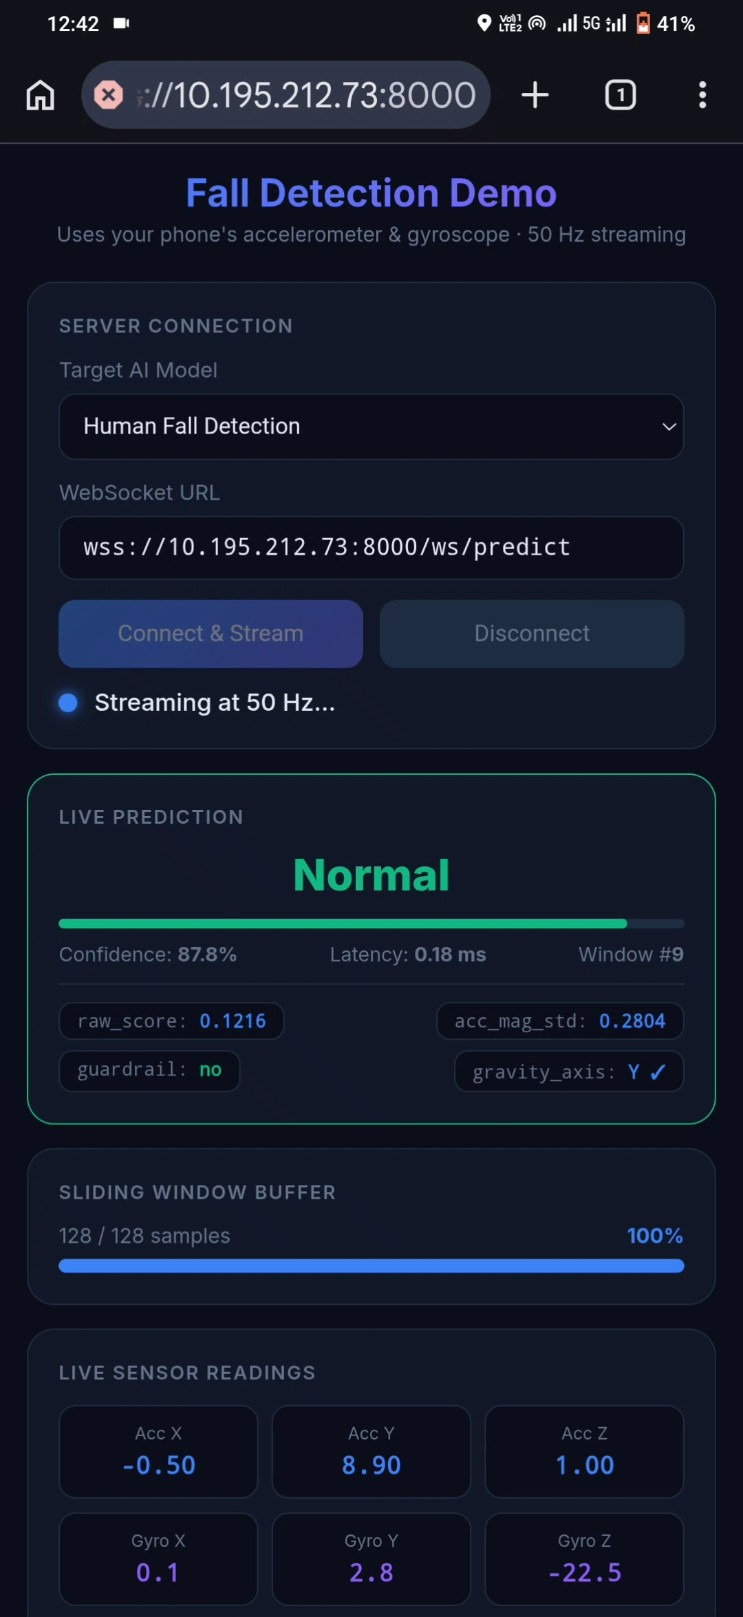
\includegraphics[width=\linewidth]{Normal_Screenshot.jpeg}
  \subcaption{Normal Activity. Confidence = 87.8\%, guardrail = off.}
\end{minipage}
\hfill
\begin{minipage}{0.48\linewidth}
  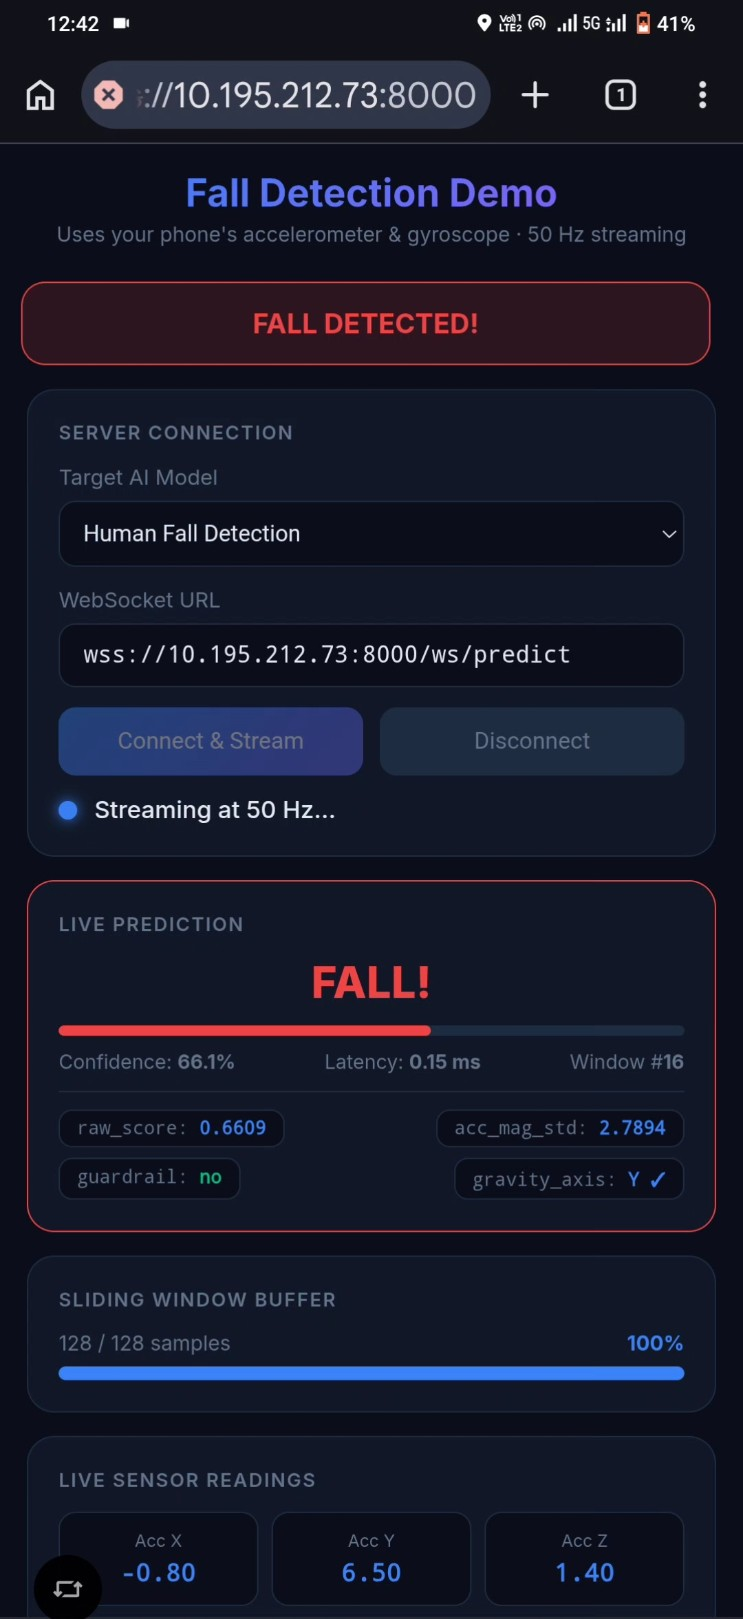
\includegraphics[width=\linewidth]{Fall_Screenshot.jpeg}
  \subcaption{Fall Detected. Confidence = 66.1\%, TFLite-only latency = 0.15~ms.}
\end{minipage}
\caption{Live mobile dashboard on an iQOO Z3 Android smartphone at 50~Hz
over Wi-Fi. The 0.15~ms shown is TFLite model-only inference latency;
full system-level latency is $\sim$2~ms (Section~\ref{sec:latency}).}
\label{fig:demo}
\end{figure}

\subsection{Comparison with State of the Art (Fall Detection Only)}

Table~\ref{tab:sota} compares our fall detection results with prior works.
No crash detection comparison is provided since the crash model was
trained on a proprietary synthetic dataset; a fair comparison requires
a common benchmark.

\begin{table}[!ht]
\renewcommand{\arraystretch}{1.3}
\caption{Comparison with Prior Work on Human Fall Detection}
\label{tab:sota}
\centering
\begin{tabular}{lcccc}
\toprule
\textbf{Reference} & \textbf{Dataset} & \textbf{Method} &
\textbf{Acc.\,(\%)} & \textbf{Edge?} \\
\midrule
\citet{kangas2008}     & Custom   & Threshold         & 95.0 & Yes \\
\citet{wang2020cnn}    & Various  & 1D-CNN            & 97.3 & Partial \\
\citet{musci2020}      & MobiFall & LSTM              & 98.1 & No \\
\citet{nho2021}        & SisFall  & Bi-LSTM           & 99.1 & No \\
\citet{mobifall2024}   & MobiFall & Lightweight CNN   & 97.8 & Partial \\
\textbf{Ours (1D-CNN)} & MobiFall & \textbf{1D-CNN + TFLite} &
  \textbf{96.65} & \textbf{Yes} \\
\bottomrule
\end{tabular}
\end{table}

Our fall detection accuracy (96.65\%) is 1.15--2.45 percentage points
below the best LSTM/Bi-LSTM results, but the 1D-CNN is fully parallelizable,
produces a model 4.3$\times$ smaller than CNN-LSTM, and runs at $\sim$2~ms
system-level latency without a cloud round-trip. To the best of our current
survey, few works jointly consider human fall and vehicular crash-like event
detection within a single inference framework that also integrates automated
SOS alerting with GPS coordinates.

% =========================================================
% SECTION VII: EDGE DEPLOYMENT
% =========================================================
\section{Edge Deployment and Practical Considerations}
\label{sec:deployment}

\subsection{TFLite Conversion}

\begin{figure}[!ht]
\centering
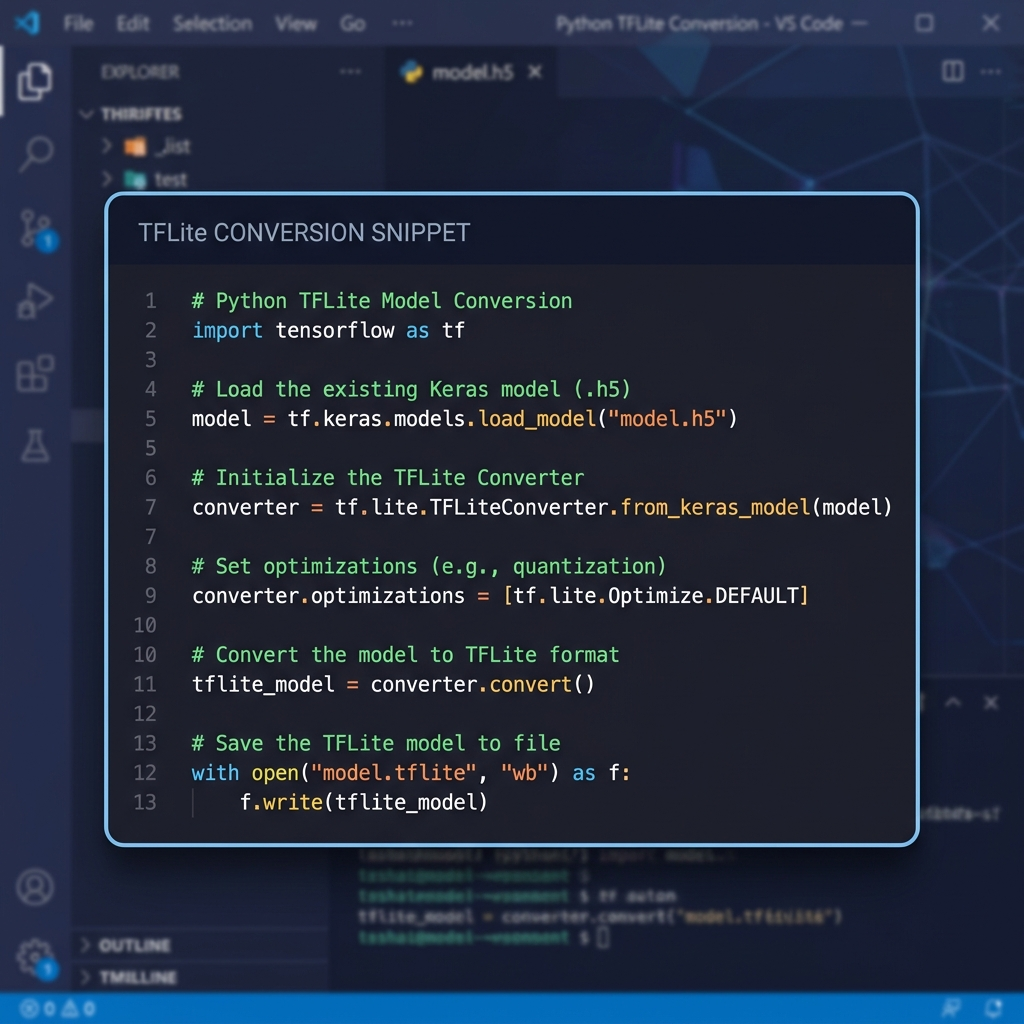
\includegraphics[width=0.95\linewidth]{tflite_conversion.png}
\caption{Core TFLite conversion code. \texttt{DYNAMIC\_RANGE} optimization
applies 8-bit quantization without a calibration dataset, achieving 88.8\%
file size reduction.}
\label{fig:tflite_code}
\end{figure}

The engine auto-detects the available TFLite runtime: \texttt{tflite\_runtime}
on Raspberry Pi~4 (ARM Cortex-A72), or the full \texttt{tensorflow} package
on a development machine, with no source code changes required.

\subsection{Sensor Orientation and Coordinate Invariance}

The acceleration magnitude $a_{\text{mag}}(t)=\sqrt{a_x^2+a_y^2+a_z^2}$
is rotation-invariant and feeds the static guardrail (Eq.~\ref{eq:guardrail}).
The neural network receives raw 6-axis channels. The MobiFall recordings span
24 subjects with varying phone positions, providing implicit orientation
robustness. The synthetic crash generator randomizes the post-crash resting
orientation matrix, exposing the crash model to varied gravitational projections.

\subsection{Limitations}
\label{sec:limitations}

\begin{enumerate}
  \item \textbf{No real crash validation.}
        The crash detection model has not been tested on any real vehicle
        crash recordings. Crash results are simulation-based feasibility
        evidence only and do not demonstrate real-world crash detection.

  \item \textbf{Synthetic crash data is simplified.}
        The generator models frontal high-G impacts followed by near-silence.
        Oblique impacts, rollovers, and multi-vehicle collisions are not
        represented. The model is expected to underperform on these cases.

  \item \textbf{Smartphone placement variability is unresolved.}
        The fall model targets the MobiFall trouser-pocket protocol.
        Dashboard mounts or hand-held positions expose different gravity axes.
        A startup calibration step has not been implemented.

  \item \textbf{Manual mode switching only.}
        Users must manually select Human Mode or Vehicle Mode. Applying the
        wrong model to the wrong context will produce incorrect predictions.

  \item \textbf{GPS may be unavailable.}
        The SOS feature depends on Geolocation permission. In tunnels or
        underground car parks, the location payload may be absent or inaccurate.

  \item \textbf{Subject-independent generalization is unconfirmed.}
        Despite the subject-wise split, the system has not been evaluated
        on a fully held-out population of new subjects.
\end{enumerate}

% =========================================================
% SECTION VIII: CONCLUSION
% =========================================================
\section{Conclusion}
\label{sec:conclusion}

This paper presented a lightweight edge-AI framework for monitoring human
passenger falls and crash-like vehicular events using the smartphone IMU.
Three aspects were demonstrated to be feasible, though significant limitations
remain before the system could be considered production-ready.

First, two independently trained binary 1D-CNN models sharing a single
hot-swappable inference engine can serve two distinct safety contexts without
the overhead of a unified multi-class model. Second, dynamic TFLite
quantization reduced each model from 137.54~KB to 15.38~KB (88.8\%
compression) with negligible accuracy loss, making deployment on
microcontroller-class hardware feasible. Third, a physics-based synthetic
generator provides a practical workaround to the near-impossibility of
obtaining labelled real crash data at scale.

On MobiFall v2.0, the 1D-CNN achieved 96.65\% fall detection accuracy with
8,481 parameters and $\sim$2~ms system-level latency, confirming that
accurate fall detection is practical on edge hardware. On the synthetic
crash dataset, the crash model achieved 93.61\% accuracy; this demonstrates
feasibility of the detection approach on synthetic data but does not
constitute evidence of real-world crash detection capability.

Work that remains: (1) validating the crash model on real recorded crash
data (e.g., NHTSA crash test sensor logs); (2) implementing automatic
context-aware mode switching; (3) evaluating on subjects not seen during
training; (4) conducting a calibration study for smartphone placement
variability. Until these steps are completed, the crash detection component
should be treated as a research prototype demonstrating feasibility, not a
validated safety-critical product.

Source code and trained models are publicly available at:\\
\url{https://github.com/DeveshNathJha/Passenger-Safety-Fall-Detection-System}

% =========================================================
% ACKNOWLEDGMENT
% =========================================================
\section*{Acknowledgment}

The authors thank the creators of MobiFall v2.0 for making their recordings
freely available. Development relied on open-source tools including TensorFlow,
Keras, FastAPI, and NumPy. Smartphone testing was carried out on an iQOO~Z3
Android device over a local Wi-Fi network.

% =========================================================
% REFERENCES
% =========================================================
\bibliographystyle{plainnat}
\bibliography{Bibliography_v2}

\end{document}
